%%%%%%%%%%%%%%%%%%%%%%%%%%%%%%%%%%%%%%%%%%%%%%%%%%%%%%%%%%%%%%%%%%
%%%%%%%%%%%%%%%%%%%%%%%%%%%%%%%%%%%%%%%%%%%%%%%%%%%%%%%%%%%%%%%%%%
%Packages
\documentclass[12pt, a4paper]{article}
\usepackage[top=3cm, bottom=4cm, left=3.2cm, right=3.2cm]{geometry}
\usepackage{amsmath,amsthm,amsfonts,amssymb,amscd, fancyhdr, comment, graphicx, environ}
\usepackage{float}
\usepackage{mathrsfs}
\usepackage{lastpage}
\usepackage[dvipsnames]{xcolor}
\usepackage[framemethod=TikZ]{mdframed}
\usepackage{enumerate}
\usepackage[shortlabels]{enumitem}
\usepackage{fancyhdr}
\usepackage{indentfirst}
\usepackage{physics}
\usepackage{textalpha}
\usepackage{amsmath}
\usepackage{amssymb}
\usepackage{sectsty}
\usepackage{thmtools}
\usepackage{shadethm}
\usepackage{hyperref}
\usepackage{setspace}
\usepackage{soul}
\hypersetup{
    colorlinks=true,
    linkcolor=blue,
    filecolor=magenta,
    urlcolor=blue,
}
\usepackage{color}
\definecolor{lightgray}{rgb}{0.95, 0.95, 0.95}
\definecolor{darkgray}{rgb}{0.4, 0.4, 0.4}
%\definecolor{purple}{rgb}{0.65, 0.12, 0.82}
\definecolor{editorGray}{rgb}{0.95, 0.95, 0.95}
\definecolor{editorOcher}{rgb}{1, 0.5, 0} % #FF7F00 -> rgb(239, 169, 0)
\definecolor{editorGreen}{rgb}{0, 0.5, 0} % #007C00 -> rgb(0, 124, 0)
\definecolor{orange}{rgb}{1,0.45,0.13}		
\definecolor{olive}{rgb}{0.17,0.59,0.20}
\definecolor{brown}{rgb}{0.69,0.31,0.31}
\definecolor{purple}{rgb}{0.38,0.18,0.81}
\definecolor{lightblue}{rgb}{0.1,0.57,0.7}
\definecolor{lightred}{rgb}{1,0.4,0.5}
\usepackage{upquote}
\usepackage{listings}
% CSS
\lstdefinelanguage{CSS}{
  keywords={color,background-image:,margin,padding,font,weight,display,position,top,left,right,bottom,list,style,border,size,white,space,min,width, transition:, transform:, transition-property, transition-duration, transition-timing-function},	
  sensitive=true,
  morecomment=[l]{//},
  morecomment=[s]{/*}{*/},
  morestring=[b]',
  morestring=[b]",
  alsoletter={:},
  alsodigit={-}
}

% JavaScript
\lstdefinelanguage{JavaScript}{
  morekeywords={typeof, new, true, false, catch, function, return, null, catch, switch, var, if, in, while, do, else, case, break},
  morecomment=[s]{/*}{*/},
  morecomment=[l]//,
  morestring=[b]",
  morestring=[b]'
}

\lstdefinelanguage{HTML5}{
  language=html,
  sensitive=true,	
  alsoletter={<>=-},	
  morecomment=[s]{<!- }{ -->},
  tag=[s],
  otherkeywords={
  % General
  >,
  % Standard tags
	<!DOCTYPE,
  </html, <html, <head, <title, </title, <style, </style, <link, </head, <meta, /, >,
	% body
	</body, <body,
	% Divs
	</div, <div, </div>, 
	% Paragraphs
	</p, <p, </p>,
	% scripts
	</script, <script,
  % More tags...
  <input, 
  <canvas, /canvas>, <svg, <rect, <animateTransform, </rect>, </svg>, <video, <source, <iframe, </iframe>, </video>, <image, </image>, <header, </header, <article, </article
  },
  ndkeywords={
  % General
  =,
  % HTML attributes
  charset=, src=, id=, width=, height=, style=, type=, rel=, href=, class=, default=, data-min=, data-max=, data-width=, data-height=,
  % SVG attributes
  fill=, attributeName=, begin=, dur=, from=, to=, poster=, controls=, x=, y=, repeatCount=, xlink:href=,
  % properties
  margin:, padding:, background-image:, border:, top:, left:, position:, width:, height:, margin-top:, margin-bottom:, font-size:, line-height:,
	% CSS3 properties
  transform:, -moz-transform:, -webkit-transform:,
  animation:, -webkit-animation:,
  transition:,  transition-duration:, transition-property:, transition-timing-function:,
  }
}

\lstdefinestyle{htmlcssjs} {%
  % General design
%  backgroundcolor=\color{editorGray},
  basicstyle={\footnotesize\ttfamily},   
  %frame=b,
  % line-numbers
  %xleftmargin={0.75cm},
  %numbers=left,
  stepnumber=1,
  firstnumber=1,
  numberfirstline=true,	
  % Code design
  identifierstyle=\color{black},
  keywordstyle=\color{blue}\bfseries,
  ndkeywordstyle=\color{editorGreen}\bfseries,
  stringstyle=\color{editorOcher}\ttfamily,
  commentstyle=\color{brown}\ttfamily,
  % Code
  language=HTML5,
  alsolanguage=JavaScript,
  alsodigit={.:;},	
  tabsize=2,
  showtabs=false,
  showspaces=false,
  showstringspaces=false,
  extendedchars=true,
  breaklines=true,
  % German umlauts
  literate=%
  {Ö}{{\"O}}1
  {Ä}{{\"A}}1
  {Ü}{{\"U}}1
  {ß}{{\ss}}1
  {ü}{{\"u}}1
  {ä}{{\"a}}1
  {ö}{{\"o}}1
}


%%%%%%%%%%%%%%%%%%%%%%%%%%%%%%%%%%%%%%%%%%%%%%%%%%%%%%%%%%%%%%%%%%
%%%%%%%%%%%%%%%%%%%%%%%%%%%%%%%%%%%%%%%%%%%%%%%%%%%%%%%%%%%%%%%%%%
%Page setup
\pagestyle{fancy}
\headheight 35pt
\rhead{
\includegraphics[width=2.5cm]{logopoli1.png}} % <-- school logo(please upload the file first, then change the name here)
\lfoot{}
\pagenumbering{arabic}
\cfoot{\small\thepage}
\rfoot{}
\headsep 3.2em
\renewcommand{\baselinestretch}{1.25}
\mdfdefinestyle{theoremstyle}{%
linecolor=black,linewidth=1pt,%
frametitlerule=true,%
frametitlebackgroundcolor=gray!20,
innertopmargin=\topskip,
}
\setlength\parskip{1em}
%%%%%%%%%%%%%%%%%%%%%%%%%%%%%%%%%%%%%%%%%%%%%%%%%%%%%%%%%%%%%%%%%%
%%%%%%%%%%%%%%%%%%%%%%%%%%%%%%%%%%%%%%%%%%%%%%%%%%%%%%%%%%%%%%%%%%
%Add new commands here
\renewcommand{\labelenumi}{\alph{enumi})}
\newcommand{\Z}{\mathbb Z}
\newcommand{\R}{\mathbb R}
\newcommand{\Q}{\mathbb Q}
\newcommand{\NN}{\mathbb N}
\DeclareMathOperator{\Mod}{Mod} 
\renewcommand\lstlistingname{Algorithm}
\renewcommand\lstlistlistingname{Algorithms}
\def\lstlistingautorefname{Alg.}
\newcommand{\quotes}[1]{``#1''}
%%%%%%%%%%%%%%%%%%%%%%%%%%%%%%%%%%%%%%%%%%%%%%%%%%%%%%%%%%%%%%%%%%
%%%%%%%%%%%%%%%%%%%%%%%%%%%%%%%%%%%%%%%%%%%%%%%%%%%%%%%%%%%%%%%%%%
%Begin now!

\begin{document}

\begin{titlepage}
    \begin{center}
        
\includegraphics[width=0.5\textwidth]{logo.png}

        \vspace*{3cm}

        \Huge
        \textbf{Granular Synthesizer}
            
        \vspace{1cm}
        \huge
        ACTaM Project\\
        \Large
        A.Y. 2021/22
            
        \vspace{1.5cm}
        
        % <-- author
        {
        \large
        \begin{tabular}{c c}
            Gargiulo Antonino Manuele & (Person code: 10829418, ID: 990594) \\
            Morena Edoardo            & (Person code: 10865449, ID: 996003) \\
            Orsatti Alessandro        & (Person code: 10680665, ID: 994757) \\
            Perego Niccolò            & (Person code: 10628782, ID: 992023)
        \end{tabular}
        }
        
            
        \vfill
        
        6 September 2022
            
        \vspace{1cm}
        
    
            
    \end{center}
\end{titlepage}


\section{Introduction}
The aim of the project was to realise a creative application involving sound. 

We focused on the development of an easy-to-use Granular Synthesizer, enriching it with multiple functionalities like the possibility to chain it with some effects, to play it using both only the mouse or with mappable MIDI controls and allowing to save and reuse some great synth configurations. 

\section{Granular Synthesis}
\subsection{An historical view}
Granular synthesis was first discussed as an outgrowth of quantum physics, when researchers such as Dennis Gabor examined the concept of reducing sound to its most basic building blocks, called \emph{sound quanta}, in the late 1940's. \newline
Gabor developed an interesting rotating tape recorder head that was able to break down the captured material into small bits for time and pitch manipulation. 

Even before computers became capable of performing the large number of calculations required to generate the necessary massive amounts of data, Iannis Xenakis both discussed and used these atomic-level sound quanta, often exploiting an enveloped simple waveform like a sine wave, or simply a bell-shaped sound impulse called \emph{wavelet}, to create statistically-shaped \emph{density clouds}, as shown in his book \quotes{Formalized Music}. 

By the time computers were ready to provide significant control to the process, leaders in the granular synthesis technique emerged in Curtis Roads and Barry Truax.
Truax was able to use his PDP minicomputer to control the grain production and results in real time. \newline The most notable musical composition realized using granular synthesis is \quotes{Riverrun} (the first word of James Joyce's \quotes{Finnegans Wake}). %At the heart of the technique is the enveloped grain, a short burst of sound that could be 10-100 milliseconds long.

Of seeming greater interest in recent decades is the granulation of real-world sampled sound. This technique was used with fascinating results in Paul Lansky's \quotes{Idle Chatter} series, circa 2011, along with several other techniques. Many DAWs, plug-ins, apps, and built-in or add-on objects for synthesis languages provide easy access to the technique both for creative and needed purposes. 

\subsection{Performing granular synthesis}
The term \quotes{granular synthesis} is rather unspecific, as it can cover all systems that utilize the concept of granulation. \textbf{Granulation} is a specific process in which an audio sample is broken down into atomomic elements, called \textbf{grains}.
A grain may have a variable length between 20 and 100 ms, where the lower bound is the integration time of the human ear (which let us differentiate sounds) while the upper bound is the limit between the granulation of a sound and a looping issue.

Generally, the original sample is split into a series of smaller ones. This original series, in chronological order, is called the \textbf{graintable}. Theoretically, if grains were played in this order at the speed of the original sample, the output would present no changes.
However we can have a lot of control over audio grains. Each one can be individually manipulated, as can the overall arrangement of them. \newline
In fact, we can play grains using different orders, individual grains can be looped, grains can be layered, omitted and skipped over. This semi-randomic process is what gives granular synthesis its distinctive feel.

After creating a new sequence of grains, volume cross-fades will be applied to blend from one gain to the next in a process called \textbf{smoothing}. The shape and length of the cross-fades have important roles in determining the tone of the resulting sound.

\section{Functionalities and Interactions}
The whole project is visually based on \emph{Bootstrap 5.0} to offer a responsive experience.

The user is firstly presented various possibilities to select the sample to be fed to the synthesizer. In fact, a dedicated area can be clicked to open a finder to select an audio file or can receive a sample drag-and-dropped on it. Lastly, the possibility to use one of the two pre-loaded default audio samples is present. \newline After this process, the main page is shown.

The first object to analyse is the \textbf{waveform visualizer}, realized with the library \emph{Wavesurfer}. The user can interact with it by selecting the point around which the granular synthesis will occur. It is also possible to move the selected point in the waveform to change the sound dynamically. \newline The last clicked position remains saved on the waveform and will be used in case the synth is played through a MIDI keyboard.

Under the waveform, the main block of \textbf{parameter knobs} is shown. This dials are the ones that act on the main characteristics of the synthesizer. In particular: 
\begin{itemize}
    \item Density: time density of the played grains;
    \item Spread: area around the waveform pointer in which the grains to be played are created;
    \item Pitch: perceived frequency of the played grains;
    \item Attack: envelope attack of each single grain;
    \item Release: envelope release of each single grain;
    \item Volume: master volume of the synthesizer.
\end{itemize}

A particular combination of values can be saved on a data base through the \quotes{Save preset} button. All the sets of parameters created by the users, along with 4 presets (designed by us) can be applied to the synthesizer picking them from a dedicated \texttt{select} element.

4 parametric effects can be dynamically toggled and operated via the GUI. In particular, the \textbf{effects and customizable values} are:

\begin{itemize}
    \item Delay
    \begin{itemize}
        \item Feedback: the amount of signal fed back to be delayed;
        \item Time: actual time delay;
    \end{itemize}
    \item Reverb
    \begin{itemize}
        \item Decay: seconds of decay of the reverb;
    \end{itemize}
    \item Distortion
    \begin{itemize}
        \item Amount: quantity of distortion applied to the grains;
    \end{itemize}
    \item LPF
    \begin{itemize}
        \item Cutoff: frequency at which the filter begins to attenuate the signal;
        \item Resonance: emphasis or suppression of portions of the signal above or below the defined cutoff frequency.
    \end{itemize}
\end{itemize}

3 \textbf{green buttons} grant the user the possibility to: reverse the current audio sample, with consequent update of the waveform, change the current audio sample and open the dynamic MIDI control assignment area. 

When shown, this last block allows the possibility to link whatever MIDI controller to one or more of the main parameters of the synthesizer.

MIDI devices are managed dynamically during the execution. They can be used to play the synthesizer using the MIDI keyboard. The pitch of the grains is modulated with respect to what key is pressed. Both this and the MIDI velocity are handled in the \emph{Granular} library.

\section{Development}
The project has been realised with HTML, JavaScript and CSS, exploiting various available libraries.

\subsection{Granular and granular\_module}
The main engine of our Granular Synthesizer is the \emph{granular-js} library, by Philipp Fromme. We locally included it in our project, in the \texttt{Granular.js} file, in order to document it and modify it to our needs. 

The \texttt{Granular} class manages the behaviour of the whole synthesis process. Actually, the \texttt{AudioContext}, the audio buffer of the loaded sample and the gain of the synth themselves are attributes of the class, used once a \texttt{Granular} object is instantiated. Another important parameter is the actual \texttt{state} of the synth, which stores the current \texttt{attack}, \texttt{release}, \texttt{pitch}, \texttt{spread} and \texttt{density} values. Lastly, an array of \texttt{Voice} objects (with respective ids), from the homonymous class, is contained in the Granular object.

The \texttt{Voice} class implements the \texttt{play} method, which is in charge of starting the synthesis process. The actual creation of the grains is done via the \texttt{createGrain} method, which is recursively called thanks to a \texttt{setTimeout} function. While creating and playing the grains, the following conditions are honored according to the choices of the user:
\begin{itemize}
    \item the right amount of time between one grain and the other (density);
    \item the right centre position in the audio buffer (where the user has clicked). The correct normalized position is received from \texttt{script.js}, where it is evaluated thanks to the \texttt{updateCursorPosition} and \texttt{normalizeTime} methods when the waveform is clicked;
    \item the proper area around the waveform pointer in which the grains to be played
    are randomly chosen (spread);
    \item the right envelope of the single grain (attack and release);
    \item the proper pitch of the grain, also taking into account the note the user has played on the MIDI keyboard if one is used;
    \item the volume, also considering the velocity if a MIDI keyboard is used.
\end{itemize}

After properly loading an audio buffer, the \texttt{startVoice} method on a \texttt{Granular} object will create a \texttt{Voice}, insert it in the \texttt{voices} array and call the \texttt{play} function on it, starting the actual sound.

When a \texttt{Voice} needs to be stopped the function \texttt{stopVoice} is called with the \texttt{Voice}'s \texttt{id} as an argument. This function also deals with the removal of the stopped \texttt{Voice} object from the \texttt{voices} array.

In the \texttt{granular\_module} script a \texttt{Granular} object is instantiated with the current \texttt{AudioContext}. Also an \texttt{Effects} object is created to manage the parametric effects to which the synth can be chained to.\newline
Some utility functions are then defined and exported to be used in \texttt{script.js} to manage the state of the \texttt{Granular} object and the whole \texttt{Effects} object.

\subsection{Audio effects: routing and typologies}
All the audio effects in our project are realized exploiting the \emph{p5.js} library. The routing follows this diagram:
\begin{figure}[h]
    \centering
    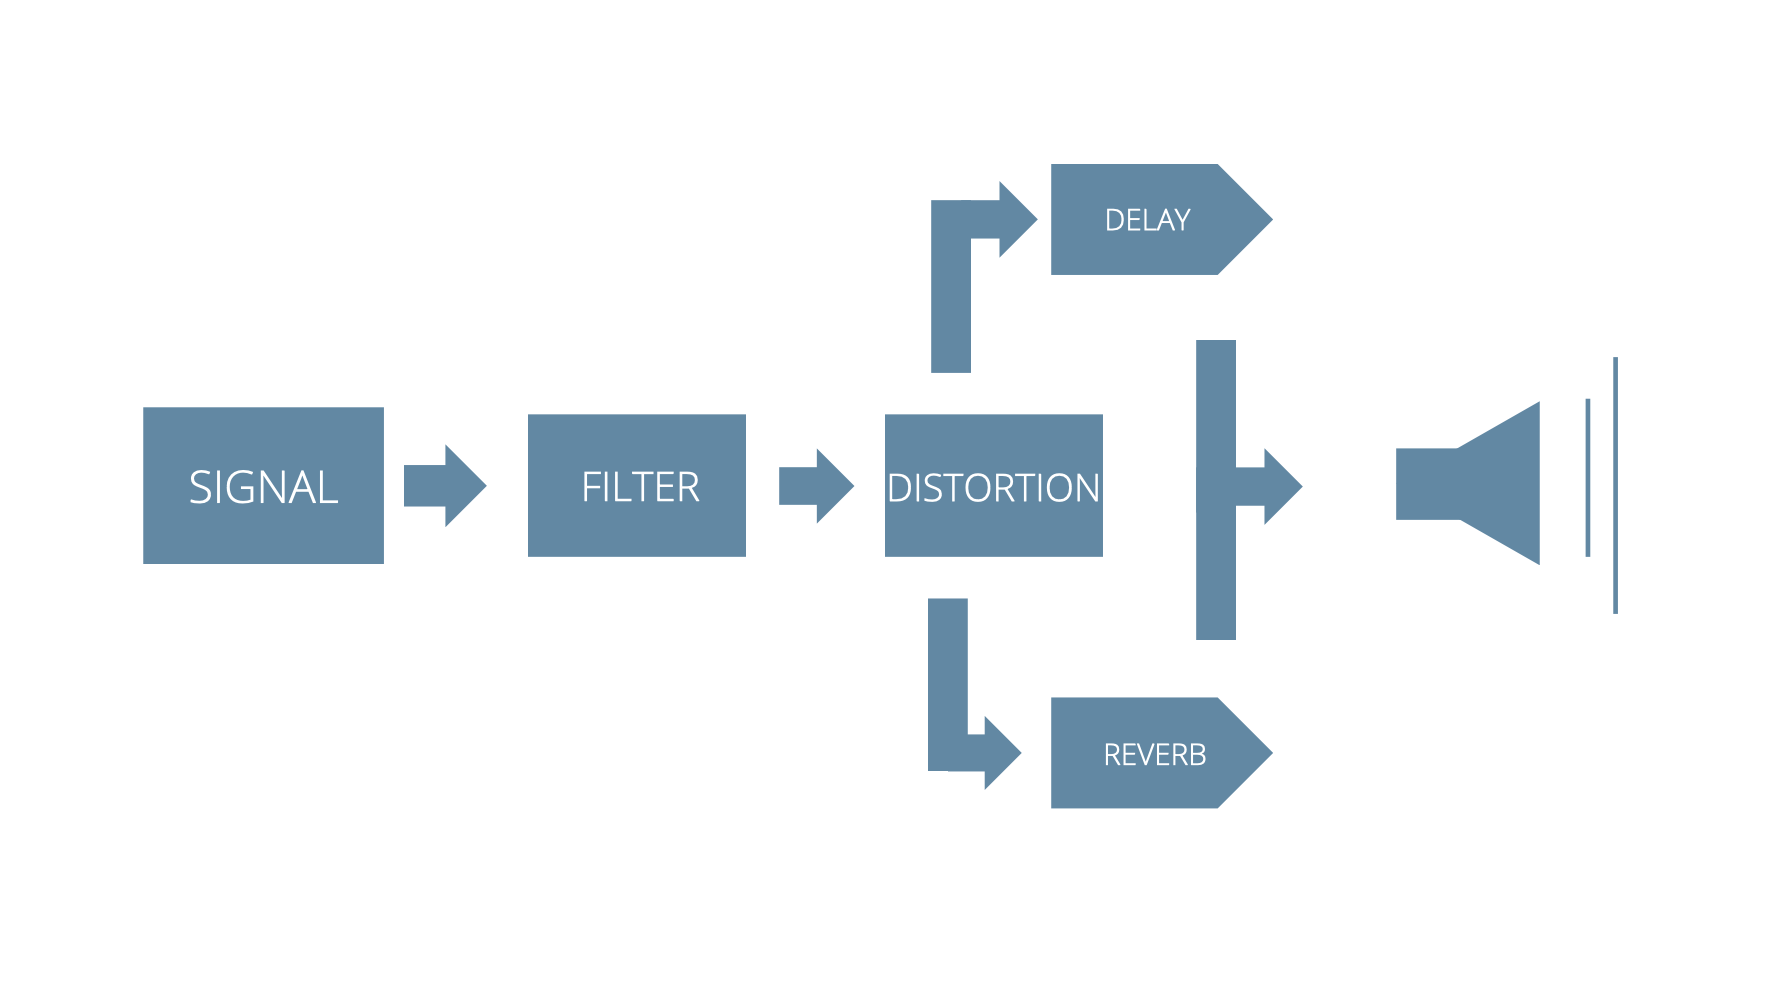
\includegraphics[scale=0.4]{effects.png}
    \caption{Effects routing}  
\end{figure}

The signal is first of all filtered with a \emph{Low Pass Filter} with parametric \texttt{cutoff} frequency and \texttt{resonance}, which output is fed into a \emph{Distortion} block, with variable \texttt{amout} of effect. Then, both a \emph{Reverb}, controlled in \texttt{decay} time, and a \emph{Delay}, with parametric \texttt{feedback} amount and \texttt{delay} time, receive the audio from the \emph{Distortion} effect and elaborate it. Finally, their output is summed and routed to the destination.

Every effect is hadled with the relative \emph{p5} object and can be switched off with a proper toggle button. For the \texttt{Distortion} and \texttt{Filter} objects, this means just selecting the respective source signal to be only sent on a dry path to bypass the effect. However, new \texttt{Reverb} and \texttt{Delay} objects need to be created and chained correctly each time the user wants to turn those effects on. 

The parameters of each effect are directly linked to the knobs present in the GUI, which trigger the update of the values both in the \texttt{Effects} object \texttt{currentState} and in the single \emph{p5} ones.

\subsection{JQuery Knobs}
We exploited the \emph{JQuery Knobs} library to create all the dials of the main page. It allows to develop canvas based elements, with no png or jpg sprites, that handle touch, mouse, mousewheel and keyboard events.

HTML elements are of the \texttt{input} type and are characterized by the class \texttt{knob}. The other classes assigned to these elements are used to style them and also serve a classification purpose in JavaScript. Each one of this elements has some special parameters which set their height, width, min, max and default values.

\vspace{0.5cm}
\begin{lstlisting}[style=htmlcssjs]
<input id="density-knob" class="knob knob-font-big par-knob animated" default="0.5" data-min="0" data-max="1" data-width="140" data-height="140" />
\end{lstlisting}

Each dial is then initialized in \texttt{script.js}. Every knob is firstly selected through \emph{JQuery} and then shaped with the method \texttt{knob}, which sets its main style and function properties, interpreting both the data fields specified in HTML and JS:

\vspace{0.5cm}
\begin{lstlisting}[style=htmlcssjs]
$('.knob').each(function () {
    var $this = $(this);
    $this.knob({
        'step': 0.01,
        'angleArc': 270,
        'angleOffset': -135,
        'lineCap': 'round',
        'fgColor': '#33383a',
    });
});
\end{lstlisting}

\noindent Properties that are specific to a certain class of knobs (or even to single ones), e.g. the change event, are then set using the \texttt{trigger} method with the \texttt{configure} setting:

\vspace{0.5cm}
\begin{lstlisting}[style=htmlcssjs]
$this.trigger(
    'configure',
    {
        'change': function (v) {
            updateGranParValue(elementId, v);
        },
        'release': function (v) {
            updateGranParValue(elementId, v);
        }, 
    }
);
\end{lstlisting}

Both the \texttt{change} and \texttt{release} properties need to be set to grant the possibility to update the knob value both with clicking and scrolling. Depending on the purpose of the dial, different exposed methods from \texttt{granular\_module} are used to update the \texttt{Granular} object \texttt{state} and the \texttt{Effect} object, which compose the model of our application.

Parameter knobs are given the \texttt{animated} class, used to recall them when the application stars or when a set of parameters is selected by the user, in order to make the visualized data swing to the correct one. This is done through the \texttt{animateToValue} and \texttt{animateToDefaultValue} methods.

\subsection{Firebase}
\emph{Firestore} is a non-relational data base offered by the \emph{Firebase} library. In our application it is used to have persistency both on default presets and on the sets of parameters created by the users. For each saved entry, a document is present in one of the 3 \emph{Firestore} collections:
\begin{itemize}
    \item \texttt{presets}: which contains all 4 presets chosen by us (plus the default one);
    \item \texttt{user\_presets}: which contains all sets of parameters saved by the users;
    \item \texttt{preset\_num}: which contains the number of saved user sets.
\end{itemize}

The first time the main page is loaded, \texttt{populatePresetList} is used to insert in the \texttt{preset-select} HTML element all the combinations of values contained in the \texttt{presets} collection. Then, the same is done for \texttt{user\_presets}, using \texttt{populatePresetListUser}. 

To keep track of the up to date number of sets created by the users and to correctly name new ones (without overrinding the contemporary creation of other sets by other users) a counter is stored in the \texttt{preset\_num} collection. \newline This value is also used to update only the changing part of the list of sets, each time a new sample is loaded (or the entire web page is refreshed).

When a user wants to save its own set of values, the listener of the click event of the \texttt{save-preset} button requests the current number of sets on the DB using \texttt{getCurrNumOfPresets}. Then, the \texttt{Granular} state is gathered with the exposed method  \texttt{getState} from \texttt{granular\_module}, and then a new document is created and saved in the \texttt{user\_presets} collection. Following this process, the list of sets in the dedicated select is updated. 

\section{Conclusion}
The achieved results fills the specifications we planned for the project and allowed us to acquire important knowledge on the synthesis topic, and also to further develop our skills in programming, following a newly found creative mind-set. 

Further work on the project might include: 
\begin{itemize}
    \item allowing the user to save each preset with a specific name;
    \item using an authentication service to offer a unique experience to each user;
    \item adding the possibility to operate effect parameters with MIDI controls.
\end{itemize}

\end{document}